\chapter{The Examination}

No sooner had Villefort left the salon, than he assumed the grave air
of a man who holds the balance of life and death in his hands. Now, in
spite of the nobility of his countenance, the command of which, like a
finished actor, he had carefully studied before the glass, it was by no
means easy for him to assume an air of judicial severity. Except the
recollection of the line of politics his father had adopted, and which
might interfere, unless he acted with the greatest prudence, with his
own career, Gérard de Villefort was as happy as a man could be. Already
rich, he held a high official situation, though only twenty-seven. He
was about to marry a young and charming woman, whom he loved, not
passionately, but reasonably, as became a deputy attorney of the king;
and besides her personal attractions, which were very great,
Mademoiselle de Saint-Méran’s family possessed considerable political
influence, which they would, of course, exert in his favor. The dowry
of his wife amounted to fifty thousand crowns, and he had, besides, the
prospect of seeing her fortune increased to half a million at her
father’s death. These considerations naturally gave Villefort a feeling
of such complete felicity that his mind was fairly dazzled in its
contemplation.

At the door he met the commissary of police, who was waiting for him.
The sight of this officer recalled Villefort from the third heaven to
earth; he composed his face, as we have before described, and said, “I
have read the letter, sir, and you have acted rightly in arresting this
man; now inform me what you have discovered concerning him and the
conspiracy.”

“We know nothing as yet of the conspiracy, monsieur; all the papers
found have been sealed up and placed on your desk. The prisoner himself
is named Edmond Dantès, mate on board the three-master the \textit{Pharaon},
trading in cotton with Alexandria and Smyrna, and belonging to Morrel \&
Son, of Marseilles.”

“Before he entered the merchant service, had he ever served in the
marines?”

“Oh, no, monsieur, he is very young.”

“How old?”

“Nineteen or twenty at the most.”

At this moment, and as Villefort had arrived at the corner of the Rue
des Conseils, a man, who seemed to have been waiting for him,
approached; it was M. Morrel.

“Ah, M. de Villefort,” cried he, “I am delighted to see you. Some of
your people have committed the strangest mistake—they have just
arrested Edmond Dantès, mate of my vessel.”

“I know it, monsieur,” replied Villefort, “and I am now going to
examine him.”

“Oh,” said Morrel, carried away by his friendship, “you do not know
him, and I do. He is the most estimable, the most trustworthy creature
in the world, and I will venture to say, there is not a better seaman
in all the merchant service. Oh, M. de Villefort, I beseech your
indulgence for him.”

Villefort, as we have seen, belonged to the aristocratic party at
Marseilles, Morrel to the plebeian; the first was a royalist, the other
suspected of Bonapartism. Villefort looked disdainfully at Morrel, and
replied coldly:

“You are aware, monsieur, that a man may be estimable and trustworthy
in private life, and the best seaman in the merchant service, and yet
be, politically speaking, a great criminal. Is it not true?”

The magistrate laid emphasis on these words, as if he wished to apply
them to the owner himself, while his eyes seemed to plunge into the
heart of one who, interceding for another, had himself need of
indulgence. Morrel reddened, for his own conscience was not quite clear
on politics; besides, what Dantès had told him of his interview with
the grand-marshal, and what the emperor had said to him, embarrassed
him. He replied, however, in a tone of deep interest:

“I entreat you, M. de Villefort, be, as you always are, kind and
equitable, and give him back to us soon.” This \textit{give us} sounded
revolutionary in the deputy’s ears.

“Ah, ah,” murmured he, “is Dantès then a member of some Carbonari
society, that his protector thus employs the collective form? He was,
if I recollect, arrested in a tavern, in company with a great many
others.” Then he added, “Monsieur, you may rest assured I shall perform
my duty impartially, and that if he be innocent you shall not have
appealed to me in vain; should he, however, be guilty, in this present
epoch, impunity would furnish a dangerous example, and I must do my
duty.”

\begin{figure}[h]
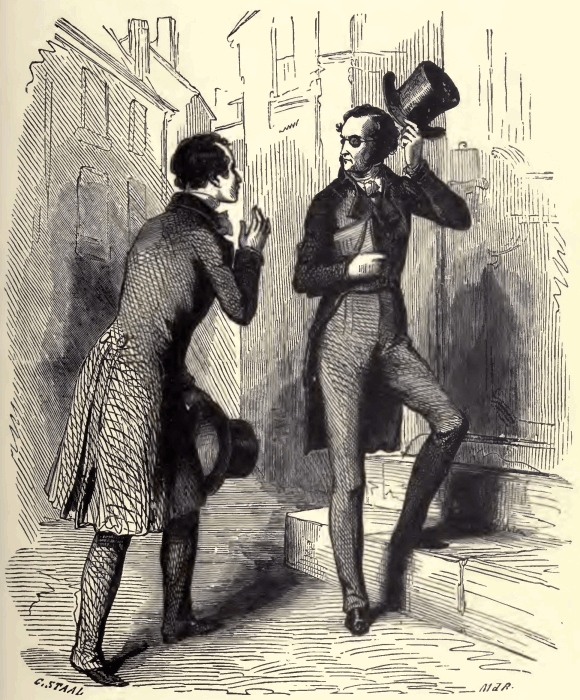
\includegraphics[width=\textwidth]{0097m.jpg}
\end{figure}

As he had now arrived at the door of his own house, which adjoined the
Palais de Justice, he entered, after having, coldly saluted the
shipowner, who stood, as if petrified, on the spot where Villefort had
left him. The antechamber was full of police agents and gendarmes, in
the midst of whom, carefully watched, but calm and smiling, stood the
prisoner. Villefort traversed the antechamber, cast a side glance at
Dantès, and taking a packet which a gendarme offered him, disappeared,
saying, “Bring in the prisoner.”

Rapid as had been Villefort’s glance, it had served to give him an idea
of the man he was about to interrogate. He had recognized intelligence
in the high forehead, courage in the dark eye and bent brow, and
frankness in the thick lips that showed a set of pearly teeth.
Villefort’s first impression was favorable; but he had been so often
warned to mistrust first impulses, that he applied the maxim to the
impression, forgetting the difference between the two words. He
stifled, therefore, the feelings of compassion that were rising,
composed his features, and sat down, grim and sombre, at his desk. An
instant after Dantès entered. He was pale, but calm and collected, and
saluting his judge with easy politeness, looked round for a seat, as if
he had been in M. Morrel’s salon. It was then that he encountered for
the first time Villefort’s look,—that look peculiar to the magistrate,
who, while seeming to read the thoughts of others, betrays nothing of
his own.

“Who and what are you?” demanded Villefort, turning over a pile of
papers, containing information relative to the prisoner, that a police
agent had given to him on his entry, and that, already, in an hour’s
time, had swelled to voluminous proportions, thanks to the corrupt
espionage of which “the accused” is always made the victim.

“My name is Edmond Dantès,” replied the young man calmly; “I am mate of
the \textit{Pharaon}, belonging to Messrs. Morrel \& Son.”

“Your age?” continued Villefort.

“Nineteen,” returned Dantès.

“What were you doing at the moment you were arrested?”

“I was at the festival of my marriage, monsieur,” said the young man,
his voice slightly tremulous, so great was the contrast between that
happy moment and the painful ceremony he was now undergoing; so great
was the contrast between the sombre aspect of M. de Villefort and the
radiant face of Mercédès.

“You were at the festival of your marriage?” said the deputy,
shuddering in spite of himself.

“Yes, monsieur; I am on the point of marrying a young girl I have been
attached to for three years.” Villefort, impassive as he was, was
struck with this coincidence; and the tremulous voice of Dantès,
surprised in the midst of his happiness, struck a sympathetic chord in
his own bosom—he also was on the point of being married, and he was
summoned from his own happiness to destroy that of another. “This
philosophic reflection,” thought he, “will make a great sensation at M.
de Saint-Méran’s;” and he arranged mentally, while Dantès awaited
further questions, the antithesis by which orators often create a
reputation for eloquence. When this speech was arranged, Villefort
turned to Dantès.

\begin{figure}[h]
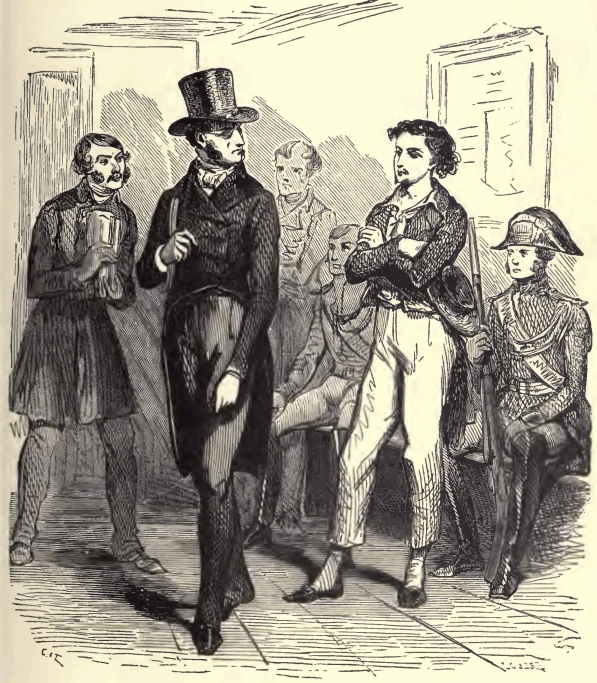
\includegraphics[width=\textwidth]{0099m.jpg}
\end{figure}

“Go on, sir,” said he.

“What would you have me say?”

“Give all the information in your power.”

“Tell me on which point you desire information, and I will tell all I
know; only,” added he, with a smile, “I warn you I know very little.”

“Have you served under the usurper?”

“I was about to be mustered into the Royal Marines when he fell.”

“It is reported your political opinions are extreme,” said Villefort,
who had never heard anything of the kind, but was not sorry to make
this inquiry, as if it were an accusation.

“My political opinions!” replied Dantès. “Alas, sir, I never had any
opinions. I am hardly nineteen; I know nothing; I have no part to play.
If I obtain the situation I desire, I shall owe it to M. Morrel. Thus
all my opinions—I will not say public, but private—are confined to
these three sentiments,—I love my father, I respect M. Morrel, and I
adore Mercédès. This, sir, is all I can tell you, and you see how
uninteresting it is.” As Dantès spoke, Villefort gazed at his ingenuous
and open countenance, and recollected the words of Renée, who, without
knowing who the culprit was, had besought his indulgence for him. With
the deputy’s knowledge of crime and criminals, every word the young man
uttered convinced him more and more of his innocence. This lad, for he
was scarcely a man,—simple, natural, eloquent with that eloquence of
the heart never found when sought for; full of affection for everybody,
because he was happy, and because happiness renders even the wicked
good—extended his affection even to his judge, spite of Villefort’s
severe look and stern accent. Dantès seemed full of kindness.

\textit{“Pardieu!”} said Villefort, “he is a noble fellow. I hope I shall gain
Renée’s favor easily by obeying the first command she ever imposed on
me. I shall have at least a pressure of the hand in public, and a sweet
kiss in private.” Full of this idea, Villefort’s face became so joyous,
that when he turned to Dantès, the latter, who had watched the change
on his physiognomy, was smiling also.

“Sir,” said Villefort, “have you any enemies, at least, that you know.”

“I have enemies?” replied Dantès; “my position is not sufficiently
elevated for that. As for my disposition, that is, perhaps, somewhat
too hasty; but I have striven to repress it. I have had ten or twelve
sailors under me, and if you question them, they will tell you that
they love and respect me, not as a father, for I am too young, but as
an elder brother.”

“But you may have excited jealousy. You are about to become captain at
nineteen—an elevated post; you are about to marry a pretty girl, who
loves you; and these two pieces of good fortune may have excited the
envy of someone.”

“You are right; you know men better than I do, and what you say may
possibly be the case, I confess; but if such persons are among my
acquaintances I prefer not to know it, because then I should be forced
to hate them.”

“You are wrong; you should always strive to see clearly around you. You
seem a worthy young man; I will depart from the strict line of my duty
to aid you in discovering the author of this accusation. Here is the
paper; do you know the writing?” As he spoke, Villefort drew the letter
from his pocket, and presented it to Dantès. Dantès read it. A cloud
passed over his brow as he said:

“No, monsieur, I do not know the writing, and yet it is tolerably
plain. Whoever did it writes well. I am very fortunate,” added he,
looking gratefully at Villefort, “to be examined by such a man as you;
for this envious person is a real enemy.” And by the rapid glance that
the young man’s eyes shot forth, Villefort saw how much energy lay hid
beneath this mildness.

“Now,” said the deputy, “answer me frankly, not as a prisoner to a
judge, but as one man to another who takes an interest in him, what
truth is there in the accusation contained in this anonymous letter?”
And Villefort threw disdainfully on his desk the letter Dantès had just
given back to him.

“None at all. I will tell you the real facts. I swear by my honor as a
sailor, by my love for Mercédès, by the life of my father——”

“Speak, monsieur,” said Villefort. Then, internally, “If Renée could
see me, I hope she would be satisfied, and would no longer call me a
decapitator.”

“Well, when we quitted Naples, Captain Leclere was attacked with a
brain fever. As we had no doctor on board, and he was so anxious to
arrive at Elba, that he would not touch at any other port, his disorder
rose to such a height, that at the end of the third day, feeling he was
dying, he called me to him. ‘My dear Dantès,’ said he, ‘swear to
perform what I am going to tell you, for it is a matter of the deepest
importance.’

“‘I swear, captain,’ replied I.

“‘Well, as after my death the command devolves on you as mate, assume
the command, and bear up for the Island of Elba, disembark at
Porto-Ferrajo, ask for the grand-marshal, give him this letter—perhaps
they will give you another letter, and charge you with a commission.
You will accomplish what I was to have done, and derive all the honor
and profit from it.’

“‘I will do it, captain; but perhaps I shall not be admitted to the
grand-marshal’s presence as easily as you expect?’

“‘Here is a ring that will obtain audience of him, and remove every
difficulty,’ said the captain. At these words he gave me a ring. It was
time—two hours after he was delirious; the next day he died.”

“And what did you do then?”

“What I ought to have done, and what everyone would have done in my
place. Everywhere the last requests of a dying man are sacred; but with
a sailor the last requests of his superior are commands. I sailed for
the Island of Elba, where I arrived the next day; I ordered everybody
to remain on board, and went on shore alone. As I had expected, I found
some difficulty in obtaining access to the grand-marshal; but I sent
the ring I had received from the captain to him, and was instantly
admitted. He questioned me concerning Captain Leclere’s death; and, as
the latter had told me, gave me a letter to carry on to a person in
Paris. I undertook it because it was what my captain had bade me do. I
landed here, regulated the affairs of the vessel, and hastened to visit
my affianced bride, whom I found more lovely than ever. Thanks to M.
Morrel, all the forms were got over; in a word I was, as I told you, at
my marriage feast; and I should have been married in an hour, and
tomorrow I intended to start for Paris, had I not been arrested on this
charge which you as well as I now see to be unjust.”

“Ah,” said Villefort, “this seems to me the truth. If you have been
culpable, it was imprudence, and this imprudence was in obedience to
the orders of your captain. Give up this letter you have brought from
Elba, and pass your word you will appear should you be required, and go
and rejoin your friends.

“I am free, then, sir?” cried Dantès joyfully.

“Yes; but first give me this letter.”

“You have it already, for it was taken from me with some others which I
see in that packet.”

“Stop a moment,” said the deputy, as Dantès took his hat and gloves.
“To whom is it addressed?”

\textit{“To Monsieur Noirtier, Rue Coq-Héron, Paris.”} Had a thunderbolt
fallen into the room, Villefort could not have been more stupefied. He
sank into his seat, and hastily turning over the packet, drew forth the
fatal letter, at which he glanced with an expression of terror.

“M. Noirtier, Rue Coq-Héron, No. 13,” murmured he, growing still paler.

“Yes,” said Dantès; “do you know him?”

“No,” replied Villefort; “a faithful servant of the king does not know
conspirators.”

\begin{figure}[h]
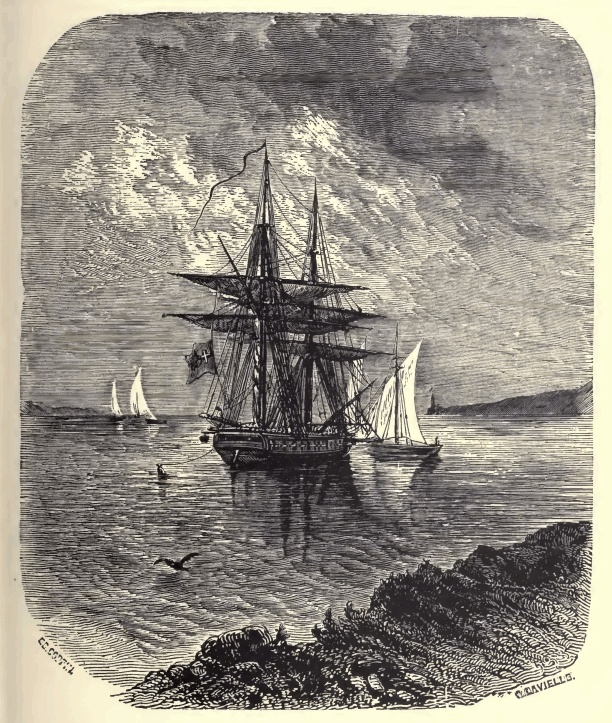
\includegraphics[width=\textwidth]{0103m.jpg}
\end{figure}

“It is a conspiracy, then?” asked Dantès, who after believing himself
free, now began to feel a tenfold alarm. “I have, however, already told
you, sir, I was entirely ignorant of the contents of the letter.”

“Yes; but you knew the name of the person to whom it was addressed,”
said Villefort.

“I was forced to read the address to know to whom to give it.”

“Have you shown this letter to anyone?” asked Villefort, becoming still
more pale.

“To no one, on my honor.”

“Everybody is ignorant that you are the bearer of a letter from the
Island of Elba, and addressed to M. Noirtier?”

“Everybody, except the person who gave it to me.”

“And that was too much, far too much,” murmured Villefort. Villefort’s
brow darkened more and more, his white lips and clenched teeth filled
Dantès with apprehension. After reading the letter, Villefort covered
his face with his hands.

“Oh,” said Dantès timidly, “what is the matter?” Villefort made no
answer, but raised his head at the expiration of a few seconds, and
again perused the letter.

“And you say that you are ignorant of the contents of this letter?”

“I give you my word of honor, sir,” said Dantès; “but what is the
matter? You are ill—shall I ring for assistance?—shall I call?”

“No,” said Villefort, rising hastily; “stay where you are. It is for me
to give orders here, and not you.”

“Monsieur,” replied Dantès proudly, “it was only to summon assistance
for you.”

“I want none; it was a temporary indisposition. Attend to yourself;
answer me.” Dantès waited, expecting a question, but in vain. Villefort
fell back on his chair, passed his hand over his brow, moist with
perspiration, and, for the third time, read the letter.

“Oh, if he knows the contents of this!” murmured he, “and that Noirtier
is the father of Villefort, I am lost!” And he fixed his eyes upon
Edmond as if he would have penetrated his thoughts.

“Oh, it is impossible to doubt it,” cried he, suddenly.

“In heaven’s name!” cried the unhappy young man, “if you doubt me,
question me; I will answer you.” Villefort made a violent effort, and
in a tone he strove to render firm:

“Sir,” said he, “I am no longer able, as I had hoped, to restore you
immediately to liberty; before doing so, I must consult the trial
justice; what my own feeling is you already know.”

“Oh, monsieur,” cried Dantès, “you have been rather a friend than a
judge.”

\begin{figure}[h]
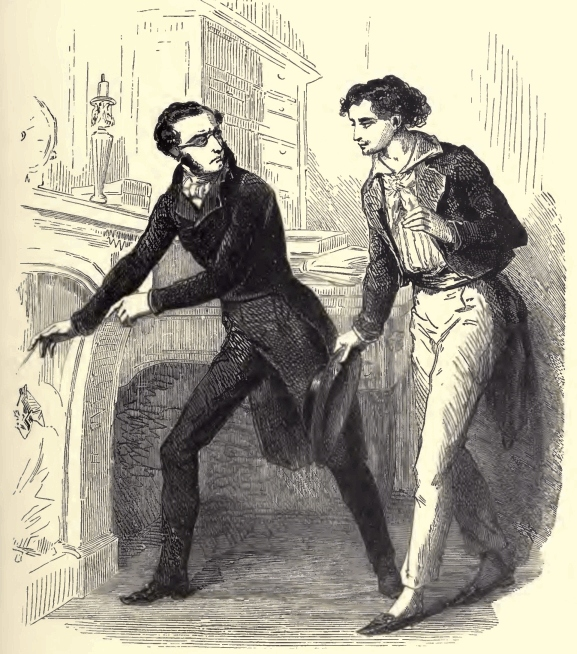
\includegraphics[width=\textwidth]{0105m.jpg}
\end{figure}

“Well, I must detain you some time longer, but I will strive to make it
as short as possible. The principal charge against you is this letter,
and you see——” Villefort approached the fire, cast it in, and waited
until it was entirely consumed.

“You see, I destroy it?”

“Oh,” exclaimed Dantès, “you are goodness itself.”

“Listen,” continued Villefort; “you can now have confidence in me after
what I have done.”

“Oh, command, and I will obey.”

“Listen; this is not a command, but advice I give you.”

“Speak, and I will follow your advice.”

“I shall detain you until this evening in the Palais de Justice. Should
anyone else interrogate you, say to him what you have said to me, but
do not breathe a word of this letter.”

“I promise.” It was Villefort who seemed to entreat, and the prisoner
who reassured him.

“You see,” continued he, glancing toward the grate, where fragments of
burnt paper fluttered in the flames, “the letter is destroyed; you and
I alone know of its existence; should you, therefore, be questioned,
deny all knowledge of it—deny it boldly, and you are saved.”

“Be satisfied; I will deny it.”

“It was the only letter you had?”

“It was.”

“Swear it.”

“I swear it.”

Villefort rang. A police agent entered. Villefort whispered some words
in his ear, to which the officer replied by a motion of his head.

“Follow him,” said Villefort to Dantès. Dantès saluted Villefort and
retired. Hardly had the door closed when Villefort threw himself
half-fainting into a chair.

“Alas, alas,” murmured he, “if the procureur himself had been at
Marseilles I should have been ruined. This accursed letter would have
destroyed all my hopes. Oh, my father, must your past career always
interfere with my successes?” Suddenly a light passed over his face, a
smile played round his set mouth, and his haggard eyes were fixed in
thought.

“This will do,” said he, “and from this letter, which might have ruined
me, I will make my fortune. Now to the work I have in hand.” And after
having assured himself that the prisoner was gone, the deputy procureur
hastened to the house of his betrothed.

\begin{figure}[h]
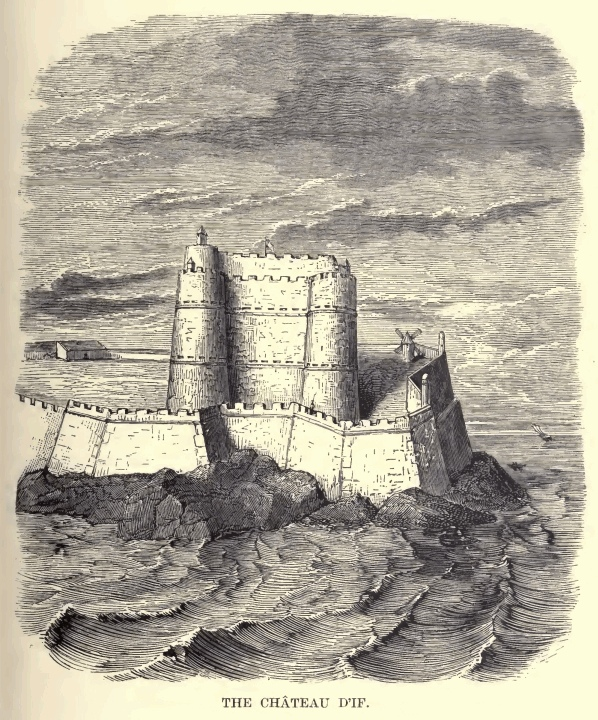
\includegraphics[width=\textwidth]{0107m.jpg}
\end{figure}
